\begin{center}
    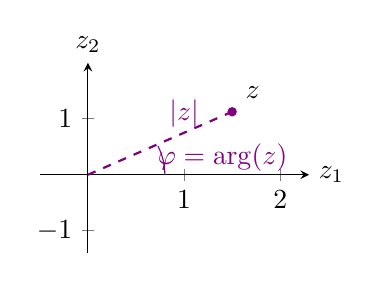
\begin{tikzpicture}
        [
            scale = 1.0,
            >=latex
        ]
        \begin{axis}[
            xmin=-0.5,
            xmax=2.3,
            ymin=-1.4,
            ymax=2,
            width=5cm,
            height=4cm,
            axis x line=middle, 
            axis y line=middle, 
            xtick={0, 1, 2},
            xticklabels={$0$, $1$, $2$},
            ytick={-1, 0, 1},
            x label style={anchor=west},
            xlabel={$z_1$}, 
            y label style={anchor=south},
            ylabel={$z_2$}
        ]
        
        \addplot[violet, dashed, thick, domain=0:1.5] {0.75*x};
        \draw[violet] (0.8, 0) arc[start angle=0, end angle=27, radius=0.8cm];
        \node[violet] at (1.4, 0.3) {$\varphi = \arg(z)$};
        
        \node[violet] at (1, 1.1) {$|z|$};

        \node[circle, fill=violet, inner sep=1.2pt, label={above right:$z$}] at (axis cs:1.5, 1.125) {};


        \end{axis}
    \end{tikzpicture}
\end{center}